\documentclass[12pt]{article}
\usepackage{epsfig}
\usepackage{graphicx}
\usepackage{color}
\usepackage[frenchb]{babel}
\usepackage{subfigure}
\usepackage{amsmath}
\usepackage{amssymb}
\usepackage{enumerate}

% Pour pouvoir utiliser les accents directement dans LaTeX, sans utiliser les commandes \'
%\usepackage[latin1]{inputenc} % entree 8 bits iso-latin1
\usepackage[utf8]{inputenc} % entree 8 bits utf8, fonctionne avec MikTeX sur Windows.
\usepackage[T1]{fontenc}      % encodage 8 bits des fontes utilisees

% Pour agrandir les marges
\addtolength{\oddsidemargin}{-.875in}
\addtolength{\evensidemargin}{-.875in}
\addtolength{\textwidth}{1.75in}
\addtolength{\topmargin}{-.875in}
\addtolength{\textheight}{1.75in}

\begin{document}
\selectlanguage{french}
\title{Introduction à la robotique mobile : travail pratique 3  \\  Date de remise : 8 décembre 2017, 23h55.}
\author{Instructeur : Philippe Giguère}

\maketitle

\section {Solution par filtre à particules (10 pts)}
Le fichier \textit{src/chariot\_filtre\_particule.py} contient le code de filtre \`a particules.

\begin{figure}[ht]
 \begin{center}
  \begin{tabular}{c}
    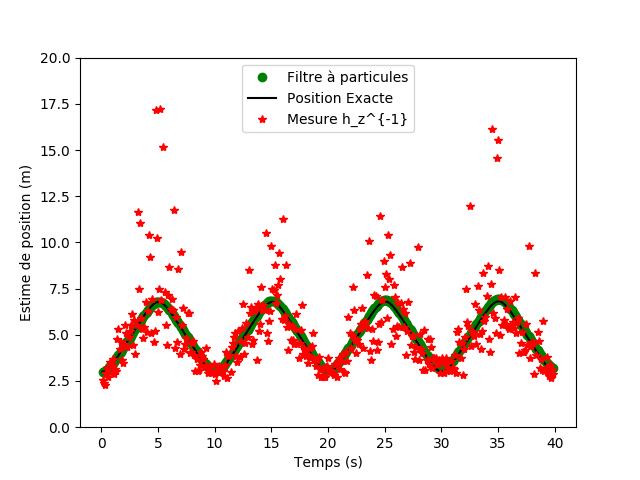
\includegraphics[width=0.75\textwidth]{fig/filtre-particule-chariot.png}
  \end{tabular}
 \end{center}
\vspace{-0.25in}
 \caption{Résultat du filtre à particules sur le chariot}
    \label{chariot-filtre-particule}
\end{figure}

La figure \ref{chariot-filtre-particule} montre le r\'esultat du filtre à particules.

\begin{figure}
\end{figure}

\section{Filtre Kalman étendu (EKF) (40 pts pour GLO-4001, 35 pts pour GLO-7021)}
\label{EKF}

\subsection{Matrices Jacobiennes (10 pts)}

\subsubsection{Détermination de $\Gamma$}
Soit nous définissons $\Gamma$ comme la matrice jacobienne des fonctions de mesure selon la commande:
\begin{equation}
\Gamma =
\begin{bmatrix}
    \dfrac{df_{position}}{du}   \\
    \\
    \dfrac{df_{vitesse}}{du}   \\
\end{bmatrix}
=
\begin{bmatrix}
    \dfrac{d}{du} \left[\dfrac{-0.07}{\alpha}\right]   \\
    \\
    \dfrac{d}{du} \left[\dfrac{2}{1+e^{-u/2}}-1\right] \\
\end{bmatrix}
\end{equation}

\begin{equation}
\Gamma =
\begin{bmatrix}
    0   \\
    \\
    \dfrac{e^{u/2}}{(1+e^{u/2})^2} \\
\end{bmatrix}
\end{equation}

\subsubsection{Détermination de $\Lambda$}
Soit nous définissons $\Lambda$ comme la matrice jacobienne des fonctions de la valeur du capteur selon les mesures.
\begin{equation}
\Lambda =
\begin{bmatrix}
    \dfrac{df_{\alpha}}{d\text{position}}  & \dfrac{df_{\alpha}}{d\text{vitesse}}
\end{bmatrix}
=
\begin{bmatrix}
    \dfrac{d}{d\text{position}} \left[\dfrac{0.07}{d}\right] & \dfrac{d}{d\text{vitesse}}\left[\dfrac{0.07}{d}\right]
\end{bmatrix}
\end{equation}

\begin{equation}
\Lambda =
\begin{bmatrix}
    \dfrac{-0.07}{d^2} & 0
\end{bmatrix}
\end{equation}

\subsection{Implémentation du filtre EKF (30 pts pour GLO-4001, 25 pts pour GLO-7021)}

Le fichier \textit{src/kalman.py} contient le code de filtre de Kalman étendu.

\subsubsection{Vous connaissez exactement la position initiale du robot au départ.}

\begin{figure}[ht]
 \begin{center}
  \begin{tabular}{c}
    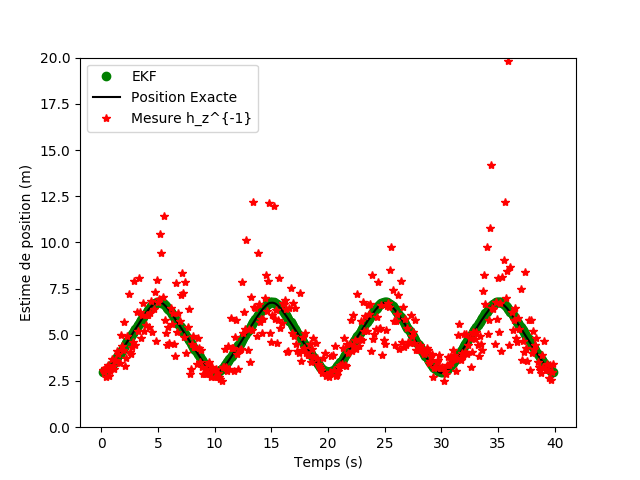
\includegraphics[width=0.75\textwidth]{fig/kalman-position-exacte.png}
  \end{tabular}
 \end{center}
\vspace{-0.25in}
 \caption{Résultat du filtre de Kalman lorsque la position de départ est exacte}
    \label{kalman-position-exacte}
\end{figure}

La figure \ref{kalman-position-exacte} présente le résultat du filtre.
Comme nous sommes certains de notre position, aucune modification n'est apporté sur le filtre.
Toutefois, comme notre position est bonne, les valeurs données par le filtre sont bonnes.


\subsubsection{Vous avez une bonne idée de la position initiale du robot au départ, mais vous n'êtes pas confiant à $100~\%$.}

\begin{figure}[ht]
 \begin{center}
  \begin{tabular}{c}
    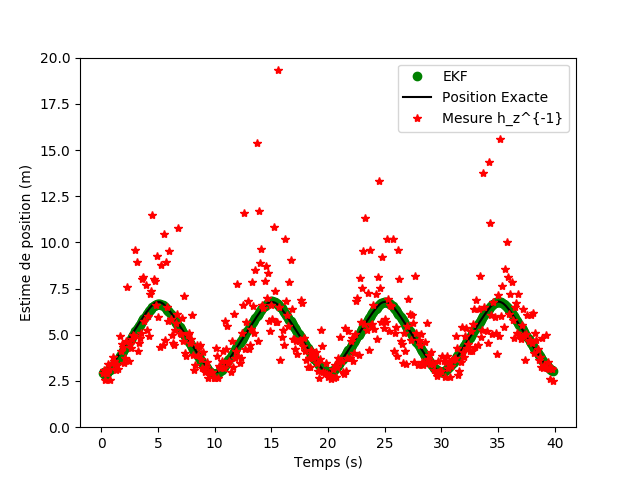
\includegraphics[width=0.75\textwidth]{fig/kalman-position-exacte-incertitude.png}
  \end{tabular}
 \end{center}
\vspace{-0.25in}
    \caption{Résultat du filtre de Kalman lorsque la position de départ est exacte, mais avec une incertitude.}
    \label{kalman-position-exacte-incertitude}
\end{figure}

La figure \ref{kalman-position-exacte-incertitude} présente le résultat du filtre.
Comme nous avons un certains niveau d'incertitude, de légères modification sont faites au filtre lors d'une différence entre les mesures et la prédiction.
Comme nous avons une bonne valeure de départ, les modifications sont minimes.

\subsubsection{Vous croyez connaitre exactement la position initiale du robot au départ, mais cette valeur est, dans les faits, erronée.}

Deux cas peuvent se produire:

\begin{figure}[ht]
 \begin{center}
  \begin{tabular}{c}
    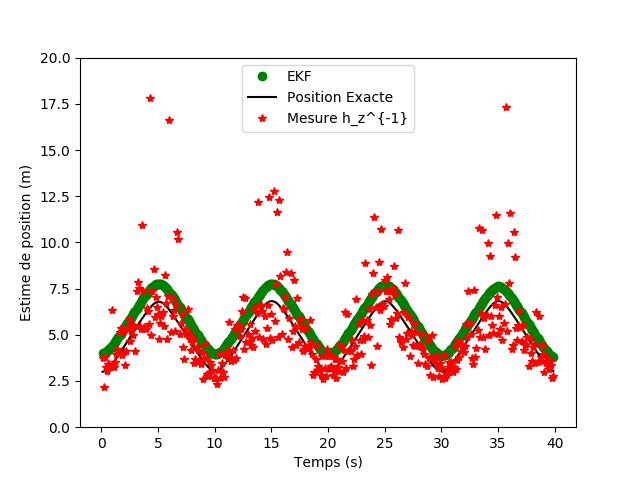
\includegraphics[width=0.75\textwidth]{fig/kalman-position-err-certitude-pas-correction.png}
  \end{tabular}
 \end{center}
\vspace{-0.25in}
    \caption{Résultat du filtre de Kalman lorsque la position de départ est considérée comme exacte, mais est fausse (sans la correction)}
    \label{kalman-position-err-certitude-pas-correction}
\end{figure}

Sans corrections, nous obtenons le résultat de la figure \ref{kalman-position-err-certitude-pas-correction}.
Comme nous avons une certitude que nous sommes au bon endroit, aucune correctionn'est fait au filtre.
Ainsi, aucune modification au gain n'est fait et la valeur du filtre a toujours une différence d'environ 1 mètre avec la vrai valeure.

\begin{figure}[ht]
 \begin{center}
  \begin{tabular}{c}
    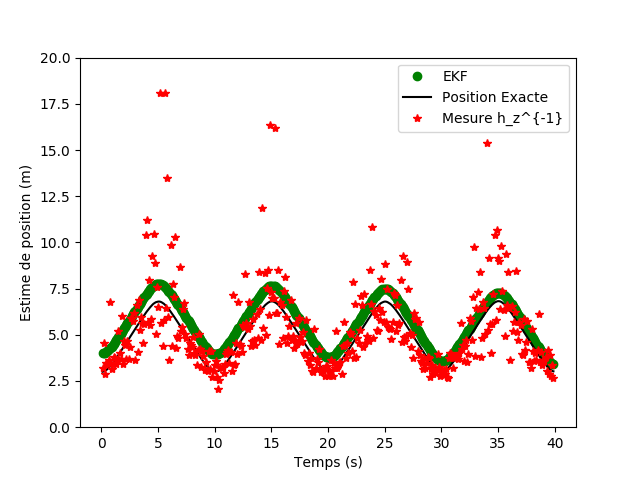
\includegraphics[width=0.75\textwidth]{fig/kalman-position-err-certitude-correction.png}
  \end{tabular}
 \end{center}
\vspace{-0.25in}
    \caption{Résultat du filtre de Kalman lorsque la position de départ est considérée comme exacte, mais est fausse (avec la correction)}
    \label{kalman-position-err-certitude-correction}
\end{figure}

Cela peut être réglée en apportant une correction à $\Gamma$.
Si l'on définit la position comme:
\begin{equation}
    d = d_{precedent} + \dot{d} \Delta t
    = d_{precedent} + \left(\dfrac{2}{1+e^{-u/2}}-1\right) \Delta t
\end{equation}
%$\alpha$ devient:
%\begin{equation}
%    \alpha = \frac{0.07}{d_{precedent} + \dot{d} \Delta t}
%\end{equation}
%
%Ce qui donne un $\Lambda$:
%
%\begin{equation}
%\Lambda =
%\begin{bmatrix}
%    \dfrac{-0.07}{(d+ \dot{d}\Delta t)^2} & \dfrac{-0.07 \Delta t}{(d+ \dot{d}\Delta t)^2}
%\end{bmatrix}
%\end{equation}

Ce qui donne un $\Gamma$:
\begin{equation}
\Gamma =
\begin{bmatrix}
    \dfrac{e^{u/2} \Delta t}{(1+e^{u/2})^2}   \\
    \\
    \dfrac{e^{u/2}}{(1+e^{u/2})^2} \\
\end{bmatrix}
\end{equation}


Nous obtenons alors la figure \ref{kalman-position-err-certitude-correction}.
Celle-ci se corrige tranquillement avec le temps.

\subsubsection{Vous n'êtes pas sûr que $d=d_{init}+1$ est la bonne position de départ du chariot.}

\begin{figure}[ht]
 \begin{center}
  \begin{tabular}{c}
    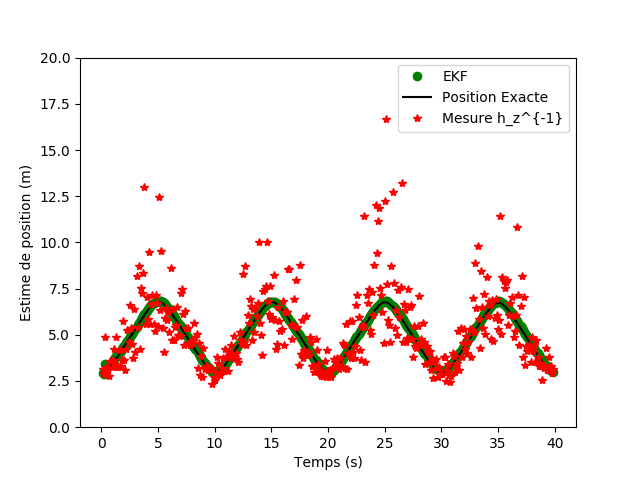
\includegraphics[width=0.75\textwidth]{fig/kalman-position-err-incertitude.png}
  \end{tabular}
 \end{center}
\vspace{-0.25in}
    \caption{Résultat du filtre de Kalman lorsque la position de départ est fausse, mais avec une incertitude.}
    \label{kalman-position-err-incertitude}
\end{figure}

La figure \ref{kalman-position-err-incertitude} présente le résultat du filtre.
Comme nous avons un certains niveau d'incertitude, de légères modification sont faites au filtre lors d'une différence entre les mesures et la prédiction.
Comme nous avons une valeure de départ érronée, les modifications sont au filtre sont plus aggressive.
Le filtre compense la différence d'environ 1 mètre entre la distance  mesurée et celle prédite.


\section {Localisation globale par filtre à particules (35 pts)}

\subsection{Cas 1 : l'angle est connu (GLO-4001 : 30 pts, GLO-7021 : 20 pts)}

\begin{itemize}
\item une justification de votre choix $\sigma_{angle}$;
\item les divers paramètres utilisés dans le filtre;
\item description qualitative de la distribution des particules au fil du temps.
\end{itemize}

\end{document}
